\documentclass[a4paper]{article}
\usepackage{a4wide,tikz}
\advance\topmargin-6\baselineskip
\advance\textheight6\baselineskip
\tikzset{gbox/.style={
    rectangle,
    draw, 
    text width=5cm,
    align=center,
    minimum height=0.8cm,
    minimum width=1.8cm
  },
  rbox/.style={gbox,rounded corners},
  confbox/.style={rbox,fill=green!40},
  subbox/.style={gbox,fill=blue!20},
  questbox/.style={gbox,fill=orange!20},
  ebox/.style={gbox,fill=red!20},
  evbox/.style={rbox,fill=green!10},
}
\begin{document}
\subsection*{Transient Absorption}
\parbox{0.5\textwidth}{%
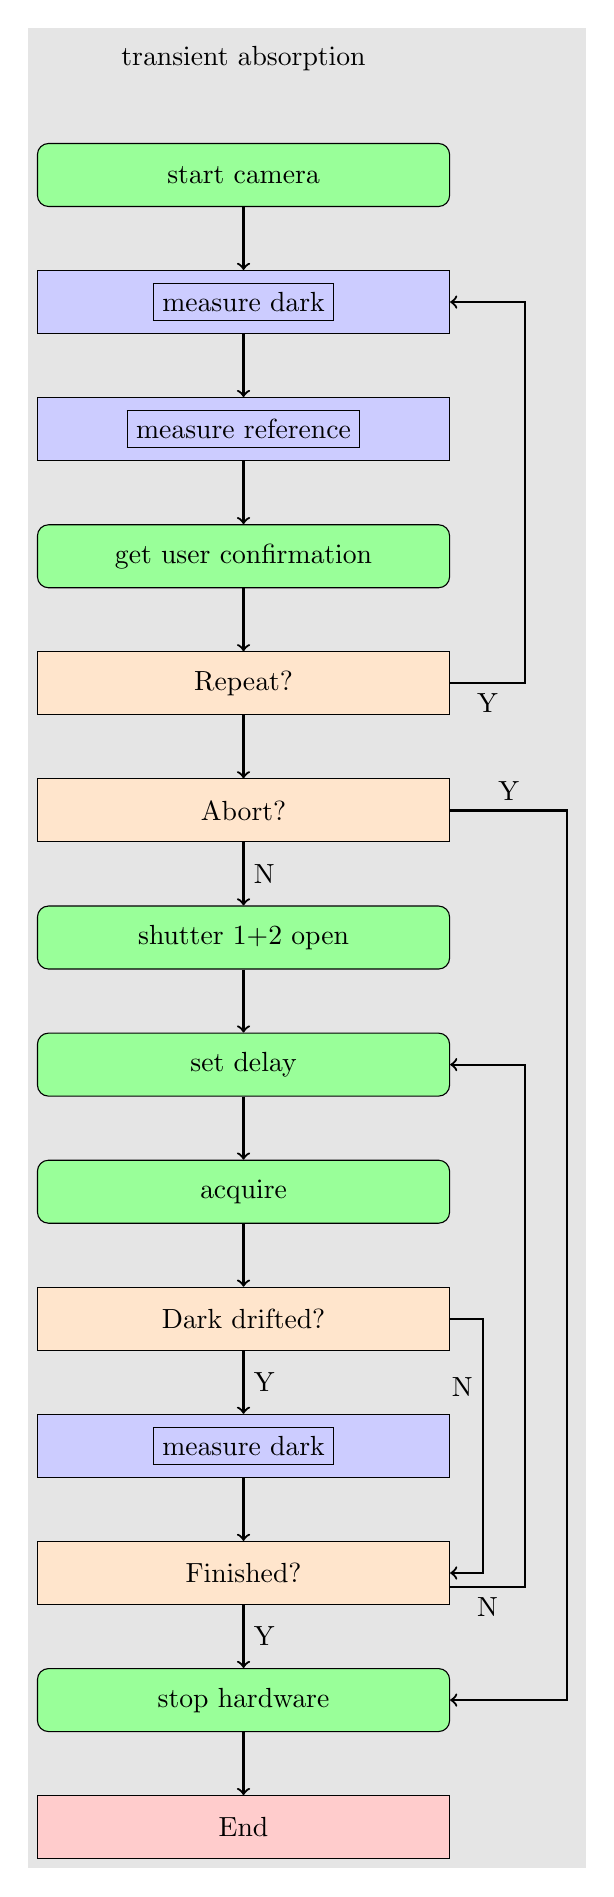
\begin{tikzpicture}[scale=0.5]
  \matrix[column sep=3mm,row sep=8mm,ampersand replacement=\&,fill=black!10] {
    \node (ta) {transient absorption}; \\
    \node [confbox] (start) {start camera}; \\
    \node [subbox] (dark) {\fbox{measure dark}}; \\
    \node [subbox] (ref) {\fbox{measure reference}}; \\
    \node [confbox] (confirm) {get user confirmation}; \\
    \node [questbox] (repeat) {Repeat?}; \& \& \node (repeat2) {}; \\
    \node [questbox] (abort) {Abort?}; \& \& \& \node (abort2) {}; \\
    \node [confbox] (prepmain) {shutter 1+2 open}; \\
    \node [confbox] (setdelay) {set delay}; \\
    \node [confbox] (acquire) {acquire}; \\
    \node [questbox] (darkok) {Dark drifted?}; \& \node (darkok2) {}; \\
    \node [subbox] (redark) {\fbox{measure dark}}; \& \node (redark2) {}; \\
    \node [questbox] (loop) {Finished?}; \& \& \node (loop2) {}; \\
    \node [confbox] (cleanup) {stop hardware}; \\
    \node [ebox] (end) {End}; \\
  };
  \draw[thick,->] (start) -- (dark);
  \draw[thick,->] (dark) -- (ref);
  \draw[thick,->] (ref) -- (confirm);
  \draw[thick,->] (confirm) -- (repeat);
  \draw[thick,->] (repeat) -- (abort);
  \draw[thick,->] (repeat) -- node [midway,below] {Y} (repeat2.center)
  |- (dark);
  \draw[thick,->] (abort) -- node [midway,right] {N} (prepmain);
  \draw[thick,->] (abort) -- node [midway,above] {Y} (abort2.center)
  |- (cleanup);
  \draw[thick,->] (prepmain) -- (setdelay);
  \draw[thick,->] (setdelay) -- (acquire);
  \draw[thick,->] (acquire) -- (darkok);
  \draw[thick,->] (darkok) -- node [midway,right] {Y} (redark);
  \draw[thick,->] (darkok) -- (darkok2.center)
  -- node [midway,left] {N} (redark2.south) |- (loop);
  \draw[thick,->] (redark) -- (loop);
  \draw[thick,->] (loop) -- node [midway,right] {Y} (cleanup);
  \draw[thick,->] ([yshift=-10]loop.east)
  -- node [midway,below] {N} ([yshift=-10]loop2.center) |- (setdelay);
  \draw[thick,->] (cleanup) -- (end);
\end{tikzpicture}}%
\parbox{0.5\textwidth}{%
\centerline{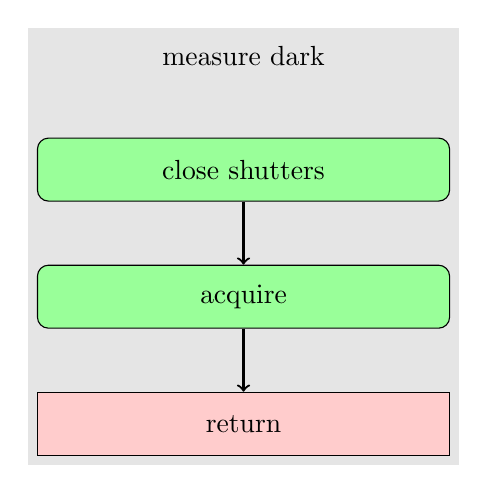
\begin{tikzpicture}[scale=0.5]
  \matrix[column sep=3mm,row sep=8mm,ampersand replacement=\&,fill=black!10] {
    \node (dark) {measure dark}; \\
    \node [confbox] (prep) { close shutters }; \\
    \node [confbox] (acquire) { acquire }; \\
    \node [ebox] (end) { return }; \\
  };
  \draw[thick,->] (prep) -- (acquire);
  \draw[thick,->] (acquire) -- (end);
\end{tikzpicture}}
\vspace{0.5cm}

\centerline{%
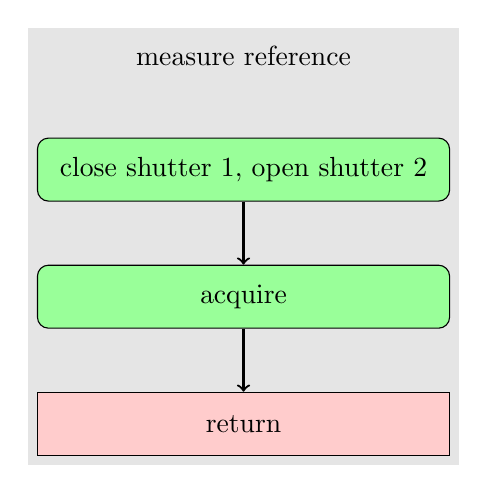
\begin{tikzpicture}[scale=0.5]
  \matrix[column sep=3mm,row sep=8mm,ampersand replacement=\&,fill=black!10] {
    \node (ref) {measure reference}; \\
    \node [confbox] (prep) { close shutter 1, open shutter 2 }; \\
    \node [confbox] (acquire) { acquire }; \\
    \node [ebox] (end) { return }; \\
  };
  \draw[thick,->] (prep) -- (acquire);
  \draw[thick,->] (acquire) -- (end);
\end{tikzpicture}}
\vspace{0.5cm}

\centerline{%
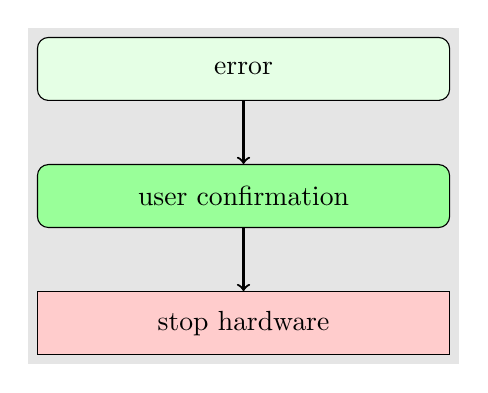
\begin{tikzpicture}[scale=0.5]
  \matrix[column sep=3mm,row sep=8mm,ampersand replacement=\&,fill=black!10] {
    \node [evbox] (error) {error}; \\
    \node [confbox] (gui) { user confirmation }; \\
    \node [ebox] (end) { stop hardware }; \\
  };
  \draw[thick,->] (error) -- (gui);
  \draw[thick,->] (gui) -- (end);
\end{tikzpicture}}
\vspace{0.5cm}

\centerline{%
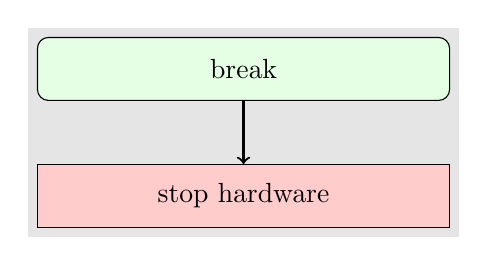
\begin{tikzpicture}[scale=0.5]
  \matrix[column sep=3mm,row sep=8mm,ampersand replacement=\&,fill=black!10] {
    \node [evbox] (break) {break}; \\
    \node [ebox] (end) { stop hardware }; \\
  };
  \draw[thick,->] (break) -- (end);
\end{tikzpicture}
}}

\subsection*{Photochemical Reaction}

\parbox{0.5\textwidth}{%
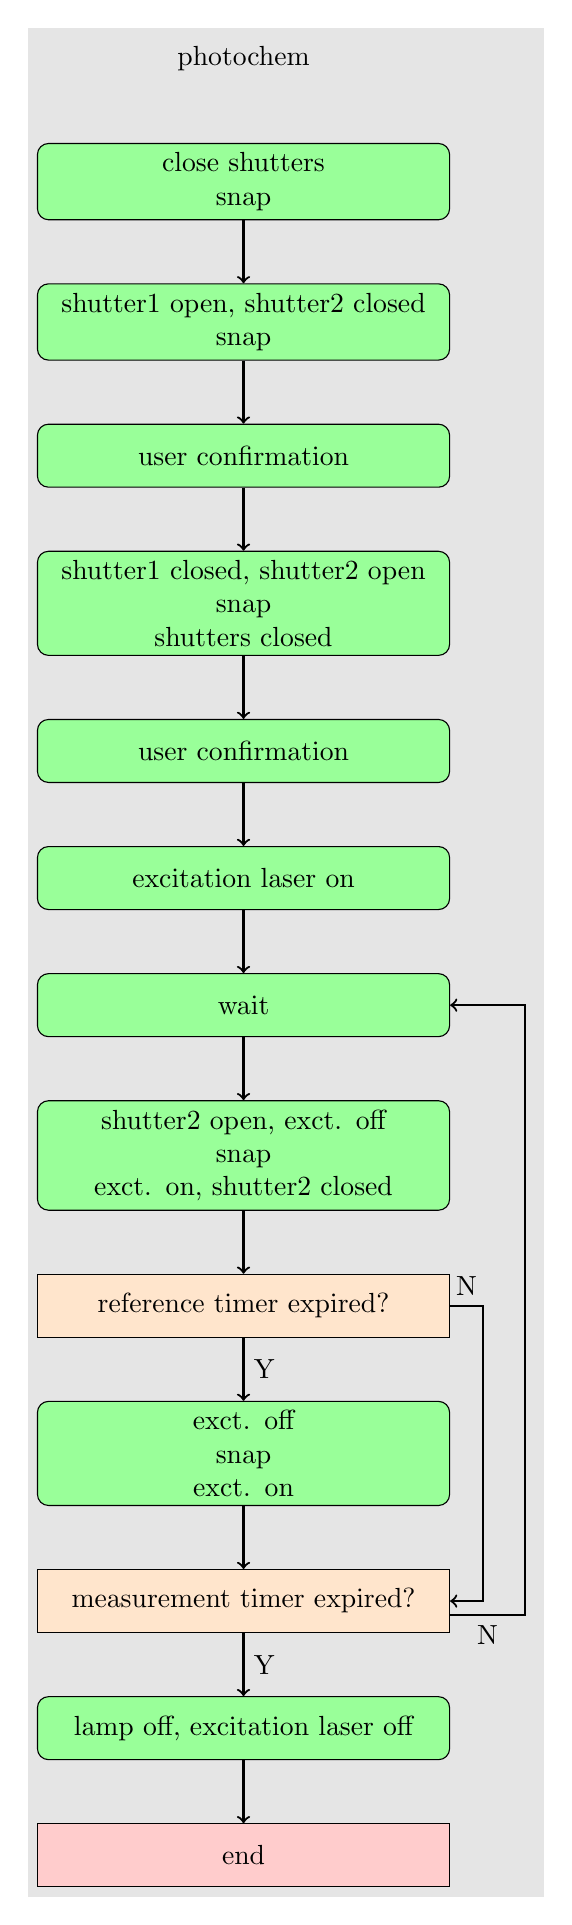
\begin{tikzpicture}[scale=0.5]
  \matrix[column sep=3mm,row sep=8mm,ampersand replacement=\&,fill=black!10] {
    \node (pchem) {photochem}; \\
    \node [confbox] (dark) {close shutters \\ snap }; \\
    \node [confbox] (ref) {shutter1 open, shutter2 closed \\ snap }; \\
    \node [confbox] (conf1) {user confirmation}; \\
    \node [confbox] (white) {shutter1 closed, shutter2 open \\ snap \\
    shutters closed}; \\
    \node [confbox] (conf2) {user confirmation}; \\
    \node [confbox] (prep) {excitation laser on}; \\
    \node [confbox] (wait) {wait}; \\
    \node [confbox] (acquire) {shutter2 open, exct. off \\ snap \\
      exct. on, shutter2 closed}; \\
    \node [questbox] (refexp) {reference timer expired?}; 
    \& \node (refexp2) {}; \\
    \node [confbox] (reref) {exct. off \\ snap \\ exct. on}; \\
    \node [questbox] (timexp) {measurement timer expired?}; 
    \& \& \node (timexp2) {}; \\
    \node [confbox] (cleanup) {lamp off, excitation laser off}; \\
    \node [ebox] (end) {end}; \\
  };
  \draw[thick,->] (dark) -- (ref);
  \draw[thick,->] (ref) -- (conf1);
  \draw[thick,->] (conf1) -- (white);
  \draw[thick,->] (white) -- (conf2);
  \draw[thick,->] (conf2) -- (prep);
  \draw[thick,->] (prep) -- (wait);
  \draw[thick,->] (wait) -- (acquire);
  \draw[thick,->] (acquire) -- (refexp);
  \draw[thick,->] (refexp) -- node [midway,right] {Y} (reref);
  \draw[thick,->] (refexp) -- node [midway,above] {N} (refexp2.center)
  |- (timexp);
  \draw[thick,->] (reref) -- (timexp);
  \draw[thick,->] (timexp) -- node [midway,right] {Y} (cleanup);
  \draw[thick,->] ([yshift=-10]timexp.east)
  -- node [midway,below] {N} ([yshift=-10]timexp2.center)
  |- (wait);
  \draw[thick,->] (cleanup) -- (end);
\end{tikzpicture}}%
\parbox{0.5\textwidth}{%
\centerline{%
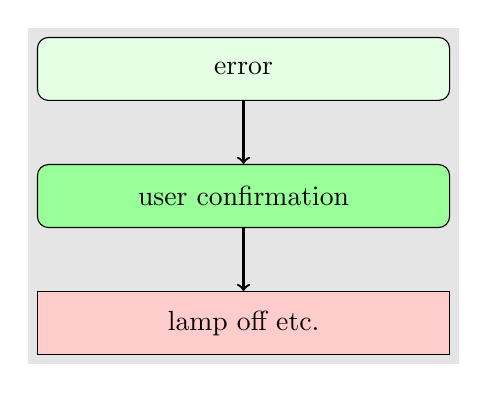
\begin{tikzpicture}[scale=0.5]
  \matrix[column sep=3mm,row sep=8mm,ampersand replacement=\&,fill=black!10] {
    \node [evbox] (error) {error}; \\
    \node [confbox] (gui) { user confirmation }; \\
    \node [ebox] (end) { lamp off etc. }; \\
  };
  \draw[thick,->] (error) -- (gui);
  \draw[thick,->] (gui) -- (end);
\end{tikzpicture}}
\vspace{0.5cm}

\centerline{%
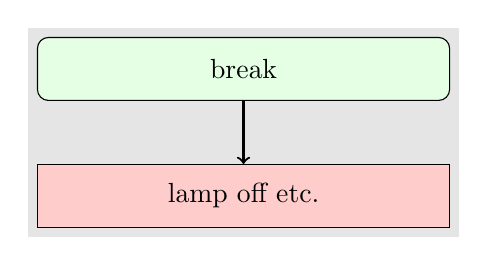
\begin{tikzpicture}[scale=0.5]
  \matrix[column sep=3mm,row sep=8mm,ampersand replacement=\&,fill=black!10] {
    \node [evbox] (break) {break}; \\
    \node [ebox] (end) { lamp off etc. }; \\
  };
  \draw[thick,->] (break) -- (end);
\end{tikzpicture}
}}

\subsection*{Temperature Dependent Absorption}

\parbox{0.5\textwidth}{%
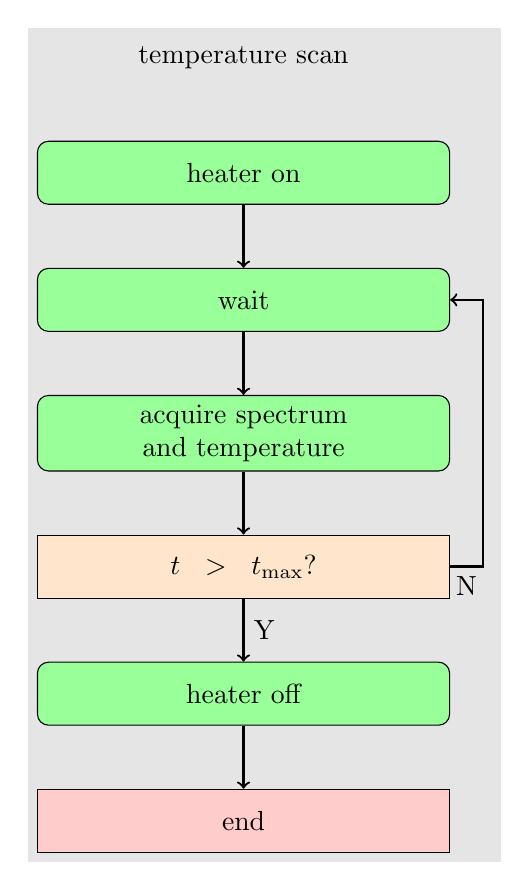
\begin{tikzpicture}[scale=0.5]
  \matrix[column sep=3mm,row sep=8mm,ampersand replacement=\&,fill=black!10] {
    \node {temperature scan}; \\
    \node [confbox] (heateron) {heater on}; \\
    \node [confbox] (wait) {wait}; \\
    \node [confbox] (acquire) {acquire spectrum and temperature}; \\
    \node [questbox] (finished) {$t>t_{\mathrm{max}}$?};
    \& \node (finished2) {}; \\
    \node [confbox] (heateroff) {heater off}; \\
    \node [ebox] (end) {end}; \\
  };
  \draw[thick,->] (heateron) -- (wait);
  \draw[thick,->] (wait) -- (acquire);
  \draw[thick,->] (acquire) -- (finished);
  \draw[thick,->] (finished) -- node [midway,right] {Y} (heateroff);
  \draw[thick,->] (finished) -- node [midway,below] {N} (finished2.center)
  |- (wait);
  \draw[thick,->] (heateroff) -- (end);
\end{tikzpicture}}%
\parbox{0.5\textwidth}{%
\centerline{%
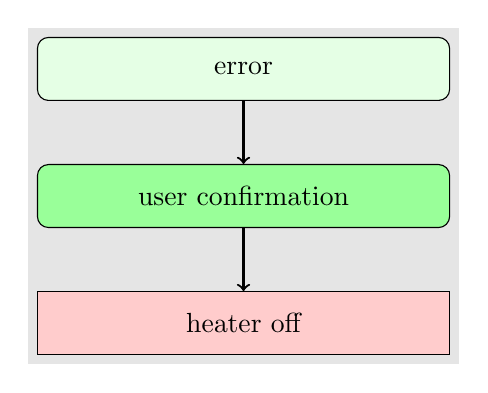
\begin{tikzpicture}[scale=0.5]
  \matrix[column sep=3mm,row sep=8mm,ampersand replacement=\&,fill=black!10] {
    \node [evbox] (error) {error}; \\
    \node [confbox] (gui) { user confirmation }; \\
    \node [ebox] (end) { heater off }; \\
  };
  \draw[thick,->] (error) -- (gui);
  \draw[thick,->] (gui) -- (end);
\end{tikzpicture}}
\vspace{0.5cm}

\centerline{%
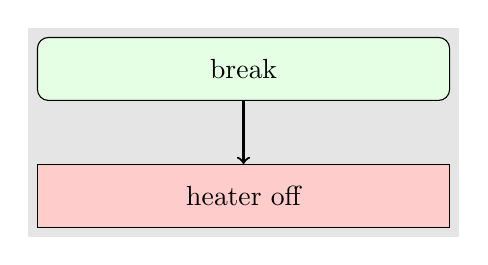
\begin{tikzpicture}[scale=0.5]
  \matrix[column sep=3mm,row sep=8mm,ampersand replacement=\&,fill=black!10] {
    \node [evbox] (break) {break}; \\
    \node [ebox] (end) { heater off }; \\
  };
  \draw[thick,->] (break) -- (end);
\end{tikzpicture}
}}


\end{document}
